\documentclass[article,shortnames,nojss]{jss}

\title{tlemix: A General Framework for Robust Fitting of Finite Mixture Models in \proglang{R}}

%\subtitle{\pkg{tlemix} version 0.2-0\\\today}

\Plaintitle{tlemix: A General Framework for Robust Fitting of Finite Mixture Models in R}
\Shorttitle{tlemix: Robust Fitting of Finite Mixture Models in \proglang{R}}

\author{Raja Patnaik, Alexander Eisl, Roland Boubela, and Peter Filzmoser\\Vienna University of Technology\\[2mm]
{\large \bf Neyko Neykov and Plamen Neytchev}\\Bulgarian Academy of Sciences}
\Plainauthor{Raja Patnaik}

\usepackage[utf8]{inputenc}
\usepackage{listings, amssymb, amsmath, graphicx}
\newcommand{\R}{\proglang{R}}


\Abstract{
  tlemix implements a general framework for robustly fitting
  discrete mixtures of regression models in the \R{} statistical
  computing environment. It implements the FAST-TLE algorithm
  and uses the R package FlexMix as a computational engine for
  fitting mixtures of general linear models (GLMs) and model-based clustering in R.
}

\Keywords{\proglang{R}, finite mixture models, model based clustering, robustness}
\Plainkeywords{R, finite mixture models, model based clustering, robustness}

\Address{
  {\bf Correspondence to:} \\
  Peter Filzmoser \\
  Department of Statistics and Probability Theory \\
  Vienna University of Technology \\
  A-1040 Vienna, Austria, Wiedner Hauptstr. 8-10 \\
  E-mail: \email{P.Filzmoser@tuwien.ac.at}\\
  URL: \url{http://statistik.tuwien.ac.at/public/filz/}
}

%%\usepackage{Sweave} %% already provided by jss.cls
%%\VignetteIndexEntry{tlemix: A General Framework for Robust Fitting of Finite Mixture Models in R}}
%%\VignetteDepends{tlemix}
%%\VignetteKeywords{R, finite mixture models, model based clustering, robustness}
%%\VignettePackage{tlemix}

\begin{document}

\section{Introduction}
\label{sec:introduction}

The initial approach to mixture analysis was first undertaken by the biometrician Karl Pearson when he was given a data set by the famous zoologist Walter Frank Raphael Weldon in 1894. In his extensive data analysis Pearson fitted a model consisting of two normal probability density functions with different means ($\mu_1$ and $\mu_2$) and different variances ($\sigma_1^2$ and $\sigma_2^2$) in proportions $\pi_1$ and $\pi_2$ to the data. Although he did not use maximum likelihood to fit the model Pearson's estimation involving the method of moments was nearly as accurate \citep[see][]{MP2000}.

Since then finite mixture models have found a variety of applications over almost 100 years, but have experienced a significant boost in popularity during the last decade as available computing power has been growing exponentially. In particular, the 1977 published approach of the EM algorithm lead to increasing interest in finite mixture models as it tremendously simplified the maximum likelihood estimation. This paper is therefore organised as follows: First the basic concept of trimmed likelihood estimation as well as the FAST-TLE algorithm implemented by tlemix are discussed. Section \ref{sec:using-tlemix} then demonstrates how to use tlemix to robustly fit finite mixture models.

% All computations and graphics in this paper have been done with
% \pkg{tlemix} version 0.0-2 and \R{} version 2.7.0 using Sweave.

\section{Trimmed Likelihood Estimator}
\label{sec:tle}

\subsection{The Weighted Trimmed Likelihood Estimator}
 Let the observations $y_1,\ldots,y_n$ denote values generated by an arbitrary probability density function $\varphi(y;\theta)$ with unknown parameter vector $\theta \in \Theta^p \subset \mathbb{R}^p$. Then, according to \cite{VN1998}, the Weighted Trimmed Likelihood Estimator (WTLE) is difined as
    \begin{equation}
    WTLE(k) (y_1,\ldots,y_n) = \hat{\theta}_{WTLE} = \arg \min_{\theta \in \Theta^p} \sum_{i=1}^k w_{\nu(i)} f(y_{\nu(i)}; \theta),\label{wtle}
    \end{equation}
where $f(y_{\nu(1)};\theta) \leq f(y_{\nu(2)};\theta) \leq \ldots \leq
f(y_{\nu(n)};\theta)$ for a fixed $\theta$,
$f(y_{i};\theta)=-\log\varphi(y_{i};\theta)$,
$y_i \in   I\hskip -3.5pt R^q$ for  $i=1,\ldots, n$ are i.i.d. observations with
probability density $\varphi(y;\theta)$, which depends on an unknown parameter
$\theta\in \Theta^{p} \subset I\hskip -3.5pt R^p$,
$\nu=(\nu(1),\ldots, \nu(n))$ is the corresponding permutation of the indices,
which depends on $\theta$, $k$ is the trimming parameter and the weights  $w_i
\ge 0$ for $i=1,\ldots,n$ are nondecreasing functions of $f(y_i,\theta)$ such
that at least $w_{\nu(k)} >0$.

The basic idea behind trimming in (\ref{wtle}) is the removal of those
$n-k$ observations whose values would be highly unlikely to occur if the fitted
model was true.

The WTLE is a combinatorial estimator according to the representation
$$
\mathop {\min }\limits_{\theta\in \Theta^{p}} \sum \limits_{i = 1}^k
w_{\nu(i)} f(y_{\nu(i)};\theta) =
\mathop {\min }\limits_{\theta\in \Theta^{p}} \mathop {\min }\limits_{I \in I_k
} \sum\limits_{i \in I} w_i f (y_i;\theta) = \mathop {\min }\limits_{I \in I_k
} \mathop {\min }\limits_{\theta\in \Theta^{p}} \sum\limits_{i \in I} w_i f
(y_i;\theta),
$$
where $I_k$ is the set of all $k$--subsets of the set $\{1,\ldots,n\}$.
Therefore, it
follows that all possible $(^{n}_{k})$ partitions of the data have to be fitted
by the MLE, and the WTLE is given by the partition with the minimal negative log likelihood.


   The WTLE accommodates different estimators depending on the weights. For instance, the median likelihood estimator MedLE(k) defined by \cite{VN1993}
   \begin{equation}
   \text{MedLE}(y_1,\ldots,y_n) = = \hat{\theta}_{MedLE} = \arg \min_{\theta \in \Theta^p} \underset{i}{\operatorname{med}} (- \ln \varphi(y_i; \theta)),\label{medle}
   \end{equation}
   is obtained by $w_{\nu(i)}=0$ for $i=1,\ldots,k-1,k+1,\ldots,n$ and $w_{\nu(k)} = 1$, and the TLE  defined by \cite{NN1990}
   \begin{equation}
   \text{TLE}(k) (y_1,\ldots,y_n) = \hat{\theta}_{TLE}= \arg \min_{\theta \in \Theta^p} \sum_{i=1}^k \left\lbrace - \ln(\varphi(y;\theta))_{(i)} \right\rbrace,\label{tle}
   \end{equation}
   is obtained if $w_{\nu(i)}=1$ for $i=1,\ldots,k$ and $w_{\nu(i)}=0$ otherwise.


\subsection{The FAST-TLE Algorithm}
\label{sec:fast-tle}

Recalling the definition of the WTLE in Eq. (\ref{wtle}) it is assumed that minimisation is achieved by subsampling the data. In view of the combinatorial nature of the algorithm, computing the WTLE for large data sets can proceed very slowly. Fortunately, an approximate algorithm called the FAST-TLE was developed by \cite{NM2003}.
The basic idea of this algorithm consists of carrying out finitely many times a two-step procedure: a trial step followed by a refinement step. In the trial step a subsample of size $k^{*}$ is selected
randomly from the data sample. The model is fitted to these $k^{*}$ observations to get $\hat{\theta^{*}}$ a trial ML estimate.  The refinement step is based on the so called concentration procedure: (a) Set $\hat{\theta}^{(c)}=\hat{\theta}^{(*)}$; (b) The cases with the $k$ smallest negative log likelihoods evaluated on the current estimate $\hat{\theta^{c}}$ are found; (b) Fitting the model to these $k$ cases gives an improved fit and let  $\hat{\theta}^{(imp)}$ be the corresponding esitmate; (c) Set $\hat{\theta}^{(c)}=\hat{\theta}^{(imp)}$. Repeating (b) and (c) yields an iterative process. The convergence is always  guaranteed after a finite number of steps since there are only finitely many $k$--subsets out of $(^{n}_{k})$.

At the end of this procedure the solution with  the lowest trimmed likelihood value is stored.  There is no guarantee that this value will be the global minimizer of (\ref{wtle}) but one can hope that it would be a close
approximation to it.
Note that in the normal linear regression and multivariate normal cases this algorithm
reduces to the concentration steps of the FAST-LTS and FAST-MCD algorithms,
respectively.

To assure the existace of a solution to the optimisation problem in Eq. (\ref{wtle}), it is assumed that $k^* \geq d$ where $d$ is the so called parameter of fulness of the set $F=\{f(y_i,\theta)=-\log\varphi(y_i;\theta), \ i=1,\ldots,n \}$.   A recommendable value of $k$ would be $\lfloor (n+d+1)/2 \rfloor$ as it would maximise the breakdown point of the WTLE estimator. Any value between $d$ and $n$ can be chosen for $k$. If the expected percentage $\alpha$ of outliers in the data is a priory known, a reasonable choice of  $k$ is $\left\lfloor n(1-\alpha) \right\rfloor$   to increase the
efficiency of the WTLE. The subsample size $k^*$ largely depends on the fullness parameter $d$ and could be defined as $k^* = d + 1$ in order to increase the chance of drawing at least one outlier free subsample \citep[see][]{NM2003}.
In the mixture setting with $g$ components, the trial sample size $k^*$ must  be at least $g(p+1)$ to overcome the degenerated case of unbounded likelihood. Thus a larger trial sample size would increase the chance to allocate at least $p+1$ cases to each mixture component. If this is not the case, any program would fail to get an estimate that could serve as a trial estimate.  If this happens a new random subsample of $k^*$ observations is drawn and supplied
to the software estimation procedure.

Since the TLE trial and refinement steps are standard MLE procedures, the
FAST-TLE algorithm can be easily implemented using widely available MLE software.
The current tlemix version employs the program FlexMix of
\cite{FL2004} and \cite{GL2008} to handle the MLE computation.
We remind that FlexMix has been developed in R ({\tt http://www.R-project.org})
as a computational engine for fitting arbitrary finite mixture models, in particular, mixtures of GLMs and model-based cluster analysis by using the EM algorithm.

%\pagebreak[4]
\section{Using tlemix}
\label{sec:using-tlemix}



As a simple example we use the artificial data set \texttt{gaussData} included in the library \texttt{tlemix} consisting of 80 observations from a mixture of two normal distributions. In order to analyse the performance of the robust FAST-TLE algorithm 20 outliers were added.

First a model framework has to be created that will be passed to the \texttt{TLE} method as the data set
\begin{Schunk}
\begin{Sinput}
> library(tlemix)
> data(gaussData)
\end{Sinput}
\end{Schunk}

We can fit this model in \R{} using the following commands:
\begin{Schunk}
\begin{Sinput}
> est.tle <- TLE(y~x,family="gaussian",data=gaussData,Density=flexmix.Density,
+ 		Estimate=flexmix.Estimate,msglvl=1,nc=2,kTrim=80,nit=10)
\end{Sinput}
\end{Schunk}
The argument \verb|kTrim=80| could be omitted, but then too many data points
would be trimmed. Moreover, the solution could be improved by increasing
the number of iterations for instance to \verb|nit=100|.
We can get a first look at the estimated parameters of mixture component~1 by
\begin{Schunk}
\begin{Sinput}
> parameters(est.tle@estimate, component=1)
\end{Sinput}
\begin{Soutput}
                     Comp.1
coef.(Intercept) -1.9632369
coef.x           -0.9709607
sigma             0.1009368
\end{Soutput}
\end{Schunk}
and
\begin{Schunk}
\begin{Sinput}
> parameters(est.tle@estimate, component=2)
\end{Sinput}
\begin{Soutput}
                    Comp.2
coef.(Intercept) 1.9712640
coef.x           0.9861527
sigma            0.1090606
\end{Soutput}
\end{Schunk}
for component~2. A cross-tabulation of true classes and cluster
memberships can be obtained by
\begin{Schunk}
\begin{Sinput}
> table(gaussData$c, est.tle@tleclusters)
\end{Sinput}
\begin{Soutput}
     1  2
  1 40  0
  2  0 40
  3  7 13
\end{Soutput}
\end{Schunk}
The summary method
\begin{Schunk}
\begin{Sinput}
> summary(est.tle)
\end{Sinput}
\begin{Soutput}
Call:
TLE(formula = y ~ x, family = "gaussian", data = gaussData, 
    kTrim = 80, nit = 10, msglvl = 1, nc = 2, Density = flexmix.Density, 
    Estimate = flexmix.Estimate)


Call:
flexmix(formula = model, data = data.frame(data), 
    k = nk, cluster = cc, model = FLXglm(model, family = family), 
    control = control)

Cluster sizes:
 1  2 
40 40 

no convergence after 2 iterations

kTrim: 80    Number of Observations: 100    Number of Outliers: 20 
\end{Soutput}
\end{Schunk}
gives the trimming parameter, the number of observations, the number of outliers and prints the \texttt{estimate} object.

Calling the summary method for the flexmix object \texttt{est.tle@estimate}
\begin{Schunk}
\begin{Sinput}
> summary(est.tle@estimate)
\end{Sinput}
\begin{Soutput}
Call:
flexmix(formula = model, data = data.frame(data), 
    k = nk, cluster = cc, model = FLXglm(model, family = family), 
    control = control)

       prior size post>0 ratio
Comp.1 0.488   40     45 0.889
Comp.2 0.512   40     47 0.851

'log Lik.' 16.79009 (df=7)
AIC: -19.58018   BIC: -2.905989 
\end{Soutput}
\end{Schunk}
displays the estimated prior probabilities $\hat\pi_k$, the
number of observations assigned to the corresponding clusters, the
number of observations where $p_{nk}>\delta$ (with a default of
$\delta=10^{-4}$), and the ratio of the latter two numbers.

For this example the method \texttt{tleplot} can be used to visualise the 2-dimensional data frame. For each cluster identified by the method \texttt{TLE} a different colour is used for indication purposes. Outliers are depicted as black triangles (see Figure \ref{fig:normal}).
\begin{Schunk}
\begin{Sinput}
> tleplot(est.tle, gaussData)
\end{Sinput}
\end{Schunk}

\begin{figure}[htbp]
  \centering
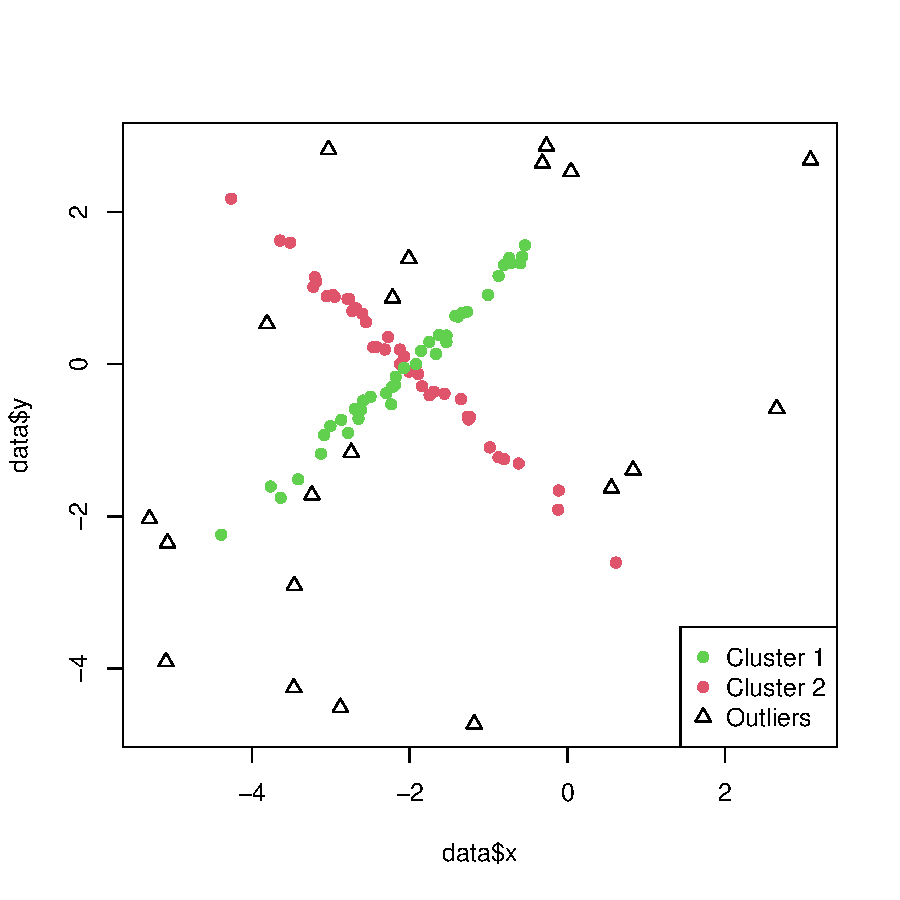
\includegraphics{tlemix-intro-010}
  \caption{Mixture of two normal components with noise. Scatterplot
  with cluster memberships.}
  \label{fig:normal}
\end{figure}

Additionally, the flexmix object can be plotted by
\begin{Schunk}
\begin{Sinput}
> plot(est.tle@estimate)
\end{Sinput}
\end{Schunk}
and will yield rootograms of the posterior class probabilities
to visually assess the cluster structure (see Figure \ref{fig:rootogram}).
\begin{figure}[htbp]
  \centering
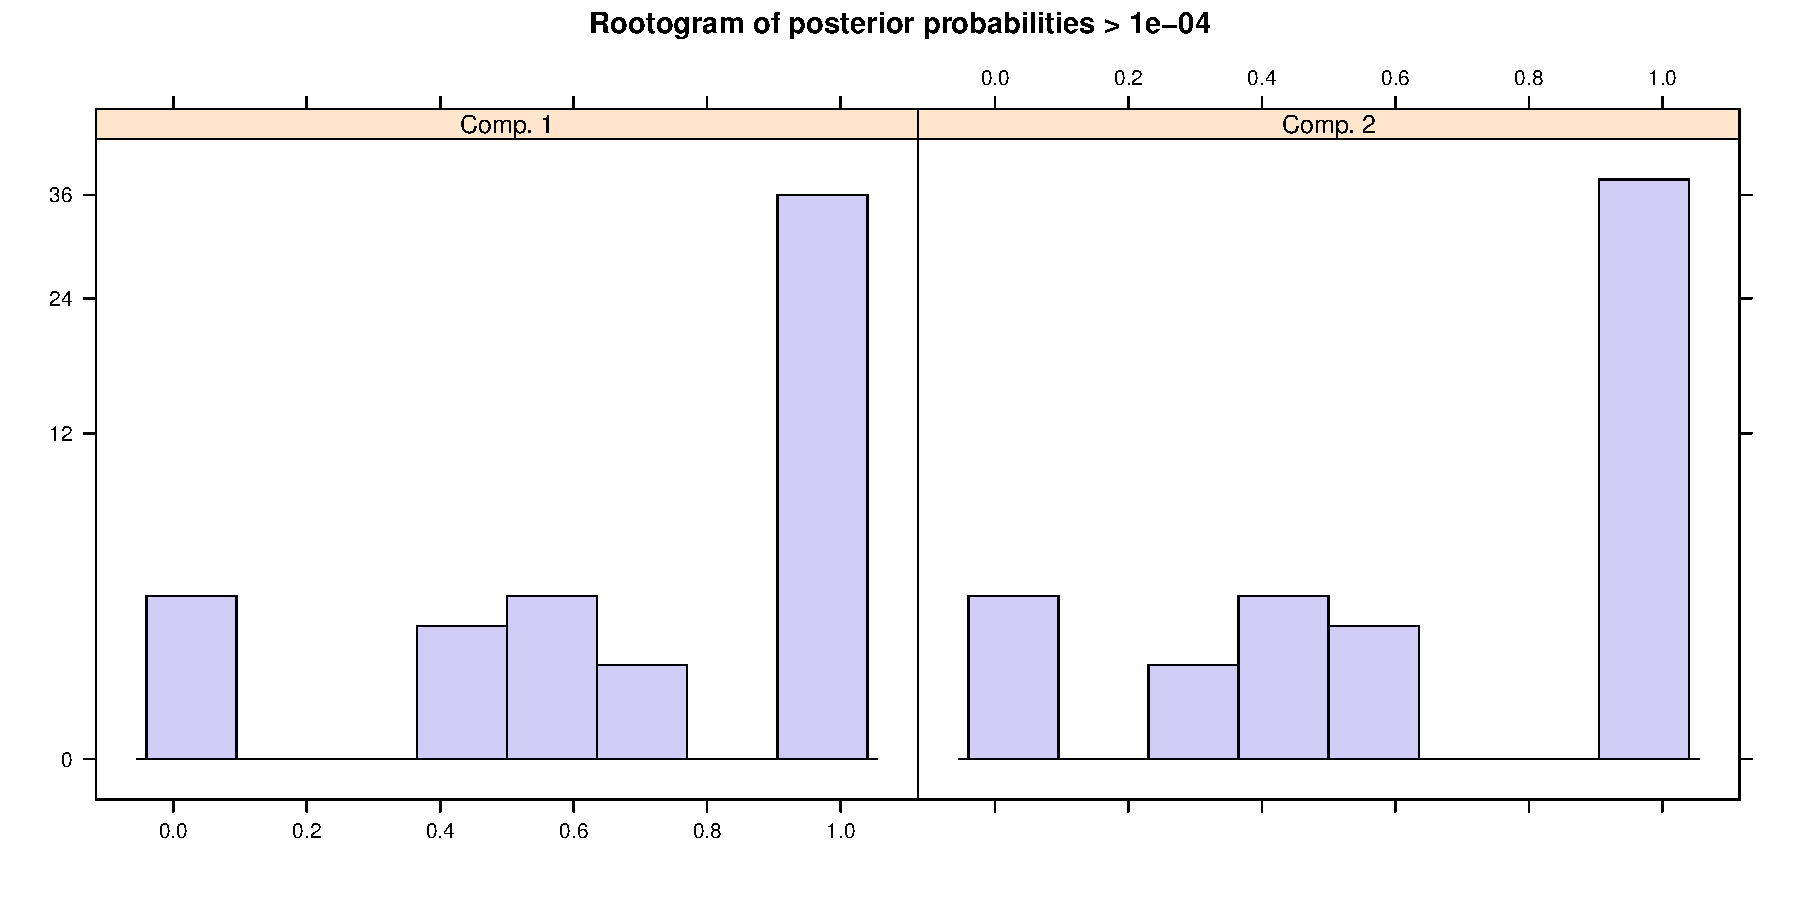
\includegraphics{tlemix-intro-012}
  \caption{Rootogram of the posterior class probabilites.}
  \label{fig:rootogram}
\end{figure}

Usually in each component a lot of observations have posteriors close
to zero, resulting in a high count for the corresponding bin in the
rootogram which obscures the information in the other bins. To avoid
this problem, all probabilities with a posterior below a threshold are
ignored (we again use $10^{-4}$).  A peak at probability 1 indicates that a
mixture component is well seperated from the other components, while
no peak at 1 and/or significant mass in the middle of the unit
interval indicates overlap with other components.

\pagebreak[4]

\bibliography{references}

\end{document}


%%% Local Variables:
%%% mode: latex
%%% TeX-master: t
%%% End:
